\def \sx {12500}
\def \sy {200000}
\def \sz {3.125\times 10^{10}}
\def \sw {50000}

\def \sa {\dfrac{13}{2500000}}
\def \sb {\dfrac{2}{25}}
\def \sc {50000}

\begin{enumerate}
	\item{
	%Part a
	\text{ }
		\begin{figure}[H]
		\begin{center}
		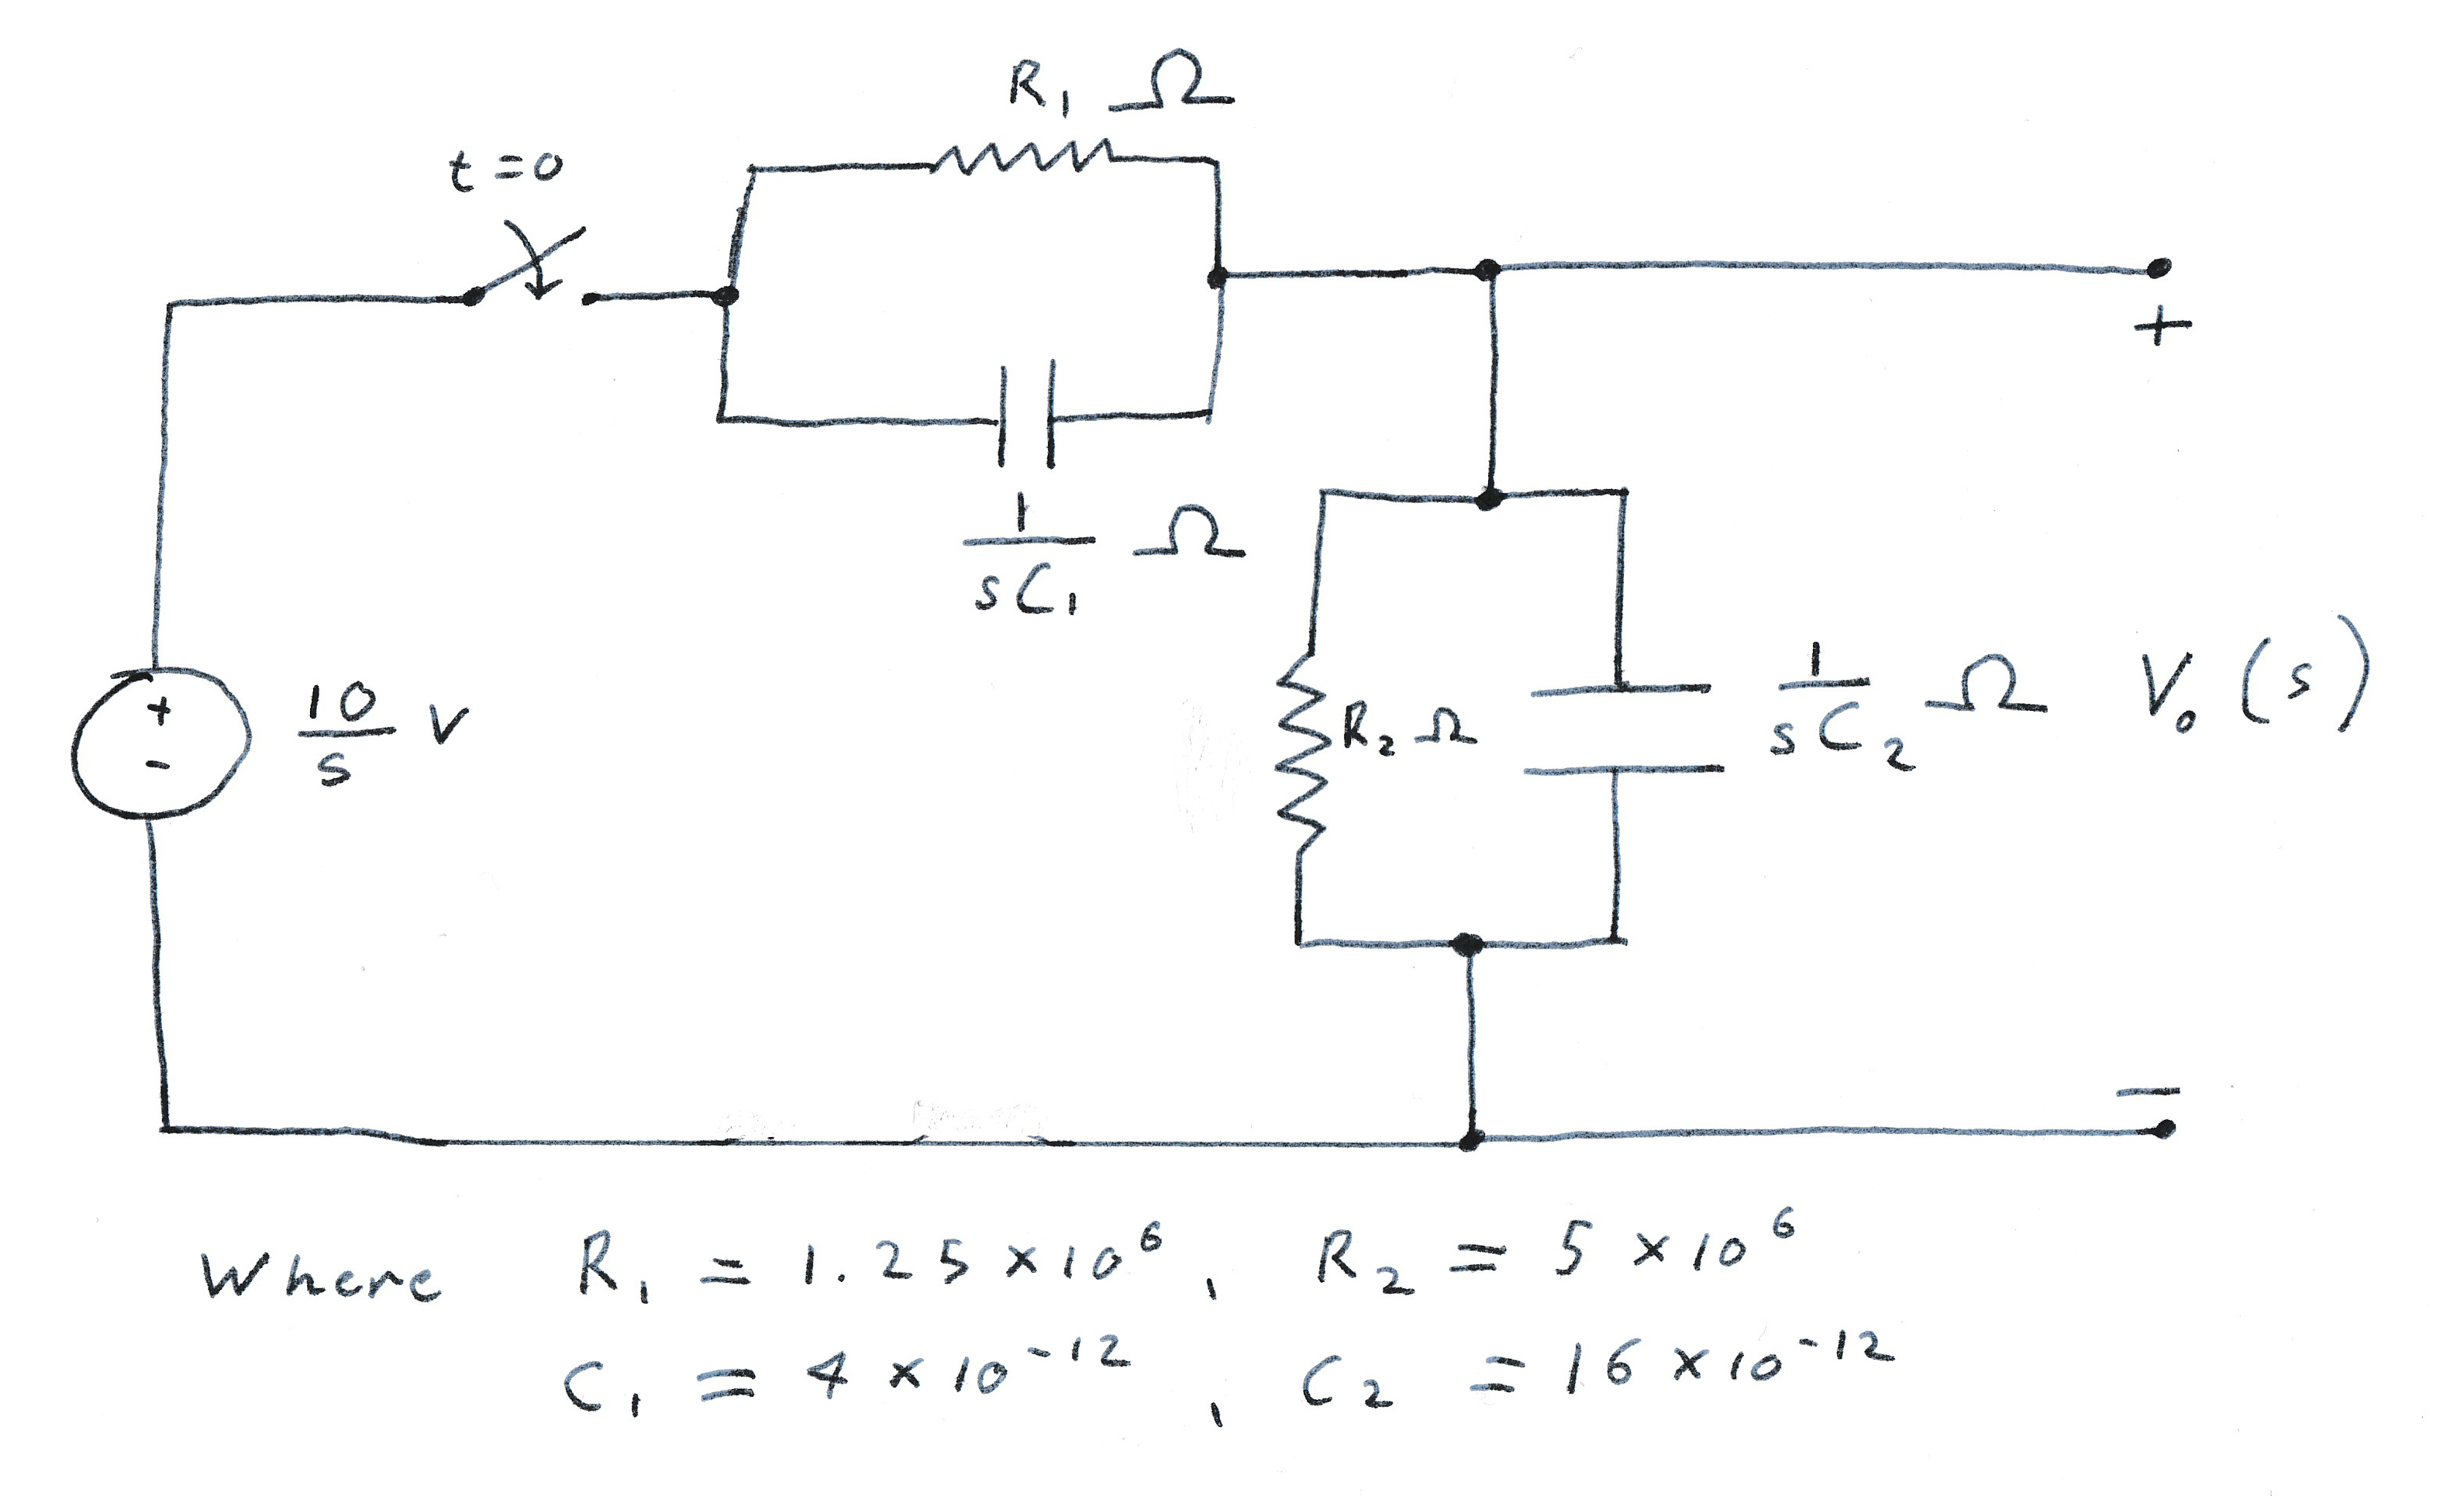
\includegraphics[scale=0.75]{1a.JPG}
		\end{center}
		\end{figure}
	}
	\item{
	%Part b
		\begin{align*}
		Z_{eq1} &= \left( \frac{1}{Z_{R_1}} +								%NEXTLINE
		\frac{1}{Z_{C_1}} \right)^{-1}\\
		&= \left( \frac{1}{R_1} + \frac{1}{\dfrac{1}{sC_1} } \right)^{-1}\\
		&= \left(\frac{1}{1.25 \times 10^6} + 								%NEXTLINE
		s \cdot 4 \times 10^{-12}\right)^{-1} \Omega\\
		&= \left(\frac{1 + 1.25\times 10^6 \cdot (s \cdot 4 \times 10^{-12})%NEXTLINE
		}{ 1.25\times 10^6} \right)^{-1} \; \Omega\\
		&= \frac{1.25\times 10^6}{1 + 1.25\times 10^6 						%NEXTLINE
		\cdot (s \cdot 4 \times 10^{-12})} \; \Omega\\
		&= \frac{2.5 \times 10^{11}}{s + 2 \times 10^5} \; \Omega
		\end{align*}
	}
	\item{
	%Part c
		\begin{align*}
		Z_{eq2} &= \left( \frac{1}{Z_{R_2}} +								%NEXTLINE
		\frac{1}{Z_{C_2}} \right)^{-1}\\
		&= \left( \frac{1}{R_2} + \frac{1}{\dfrac{1}{sC_2} } \right)^{-1}\\
		&= \left( \frac{1}{5\times 10^6} +									%NEXTLINE
		s \cdot 16 \times 10^{-12} \right)^{-1} \; \Omega\\
		&= \left( \frac{1 + 5\times 10^6 \cdot								%NEXTLINE
		(s \cdot 16 \times 10^{-12})}{5\times 10^6} \right)^{-1} \; \Omega\\
		&= \frac{5 \times 10^6}{1 + 5\times 10^6 							%NEXTLINE
		\cdot(s \cdot 16 \times 10^{-12})} \; \Omega \\
		&= \frac{6.25 \times 10^{10}}{s + 1.25 \times 10^4} \; A
		\end{align*}
	}
	\item{
	%Part d
		Using voltage division:
		\begin{align*}
		V_o(s) &= V_{in}(s) \cdot \frac{Z_{eq2}}{Z_{eq1} + Z_{eq2}}\\
		&= \frac{10}{s} \cdot \frac{\dfrac{6.25 \times 10^{10}}				%NEXTLINE
		{s + 1.25 \times 10^4}}{\dfrac{6.25 \times 10^{10}}					%NEXTLINE
		{s + 1.25 \times 10^4} + \dfrac{2.5 \times 10^{11}}					%NEXTLINE
		{s + 2 \times 10^5}} \; V\\
		&= \frac{10}{s} \cdot \frac{\dfrac{6.25 \times 10^{10}}             %NEXTLINE
		{s+1.25 \times 10^4}}{\dfrac{(6.25 \times 10^{10})					%NEXTLINE
		(s + 2\times 10^5) + (2.5 \times 10^{11})(s + 1.25 \times 10^4)}	%NEXTLINE
		{(s + 1.25 \times 10^4)\cdot(s + 2 \times 10^5)}} \; V\\
		&= \frac{10}{s} \cdot \frac{6.25 \times 10^{10}}            
		{s+1.25 \times 10^4} \cdot \frac{(s + 1.25 \times 10^4)
		\cdot(s + 2 \times 10^5)}{(6.25 \times 10^{10})
		(s + 2\times 10^5) + (2.5 \times 10^{11})
		(s + 1.25 \times 10^4)} \; V\\
		&= \frac{6.25 \times 10^{11} \cdot (s + 1.25 \times 10^4) \cdot 
		(s + 2 \times 10^5)}{3.125 \times 10^{11} \cdot s \cdot 
		(s + 1.25 \times 10^4) \cdot (s + 5 \times 10^4)} \; V\\
		&= \frac{2 \cdot (s + 2 \times 10^5)}
		{s \cdot (s + 5 \times 10^4)} \; V\\
		&= \frac{2s + 4 \times 10^5}{s^2 + 5 \times 10^4 \cdot s} \; V\\
		\end{align*}
		Using Partial fractions to continue.
		\begin{align*}
		\frac{2s + 4 \times 10^5}{s^2 + 5 \times 10^4 \cdot s} &= 
		\frac{A}{s} + \frac{B}{50000}\\
		A(s+50000) + Bs &= 2(s + 200000)\\
		(s = 0): \; 50000A &= 400000\\
		\implies A &= 8\\
		(s = -50000): \;  -50000B &= 300000\\
		B &= -6\\
		\implies V_o(s) = \frac{8}{s} - \frac{6}{s + 50000} \; V
		\end{align*}
		Using inverse Laplace transform to find $v_o(t)$.
		\begin{align*}
		v_o(t) &= \mathcal{L}^{-1} [V_o(s)]\\
		&= \mathcal{L}^{-1} \left[\frac{8}{s} - \frac{6}{s + 50000}\right]\; V\\
		&= (8 -6 e^{-50000t})u(t)\;V
		\end{align*}
	}
	\item{
	%Part e
		Using Ohm's Law in frequency domain:
		\begin{align*}
		V_{in}(s) &= Z_{eq} \cdot I_o(s)\\
		&= (Z_{eq1} + Z_{eq2}) \cdot I_o(s)\\
		\implies I_o(s) &= \frac{V_{in}(s)}{Z_{eq1} + Z_{eq2}}\\
		&= \frac{\dfrac{10}{s}} 
		{\dfrac{2.5 \times 10^{11}}
		{s + 2 \times 10^5} + \dfrac{6.25 \times 10^{10}}{s + 1.25 \times 10^4}} \; A\\
		&= \frac{\dfrac{10}{s}} 
		{\dfrac{3.125 \times 10^{11} \cdot (s + 50000)}{(s+12500)\cdot(s+200000)}} \; A\\
		&= \frac{(s+\sx)\cdot(s+\sy)}{\sz \cdot s \cdot (s + \sw)} \; A\\
		&= \frac{s^2 + s(\sx + \sy) (\sx)(\sy)}
		{\sz \cdot s^2 + s(\sz)(\sw)}\\
		&= \frac{\dfrac{s^2}{\sz} + s \dfrac{\sx + \sy}{\sz} + \dfrac{(\sx)(\sy)}{\sz}}{s^2 + s (\sw)}\\
		&= \frac{1}{\sz} + \frac{s\left(\dfrac{\sx+\sy-\sw}{\sz}\right) + \dfrac{(\sx)(\sy)}{\sz}}{s(s+\sw)}\\
		&= \frac{1}{\sz} + \frac{s \cdot \dfrac{13}{2500000} + \dfrac{2}{25} }{s(s+\sw)} 
		\end{align*}
		Use partial fraction expansion on the s term:
		
		\begin{align*}
		&\frac{A}{s} + \frac{B}{s + \sc} = \frac{\sa \cdot s + \sb}{s(s + \sc)}\\
		\implies &A(s + \sc) + B(s) = \sa \cdot s + \sb\\
		(s = 0) \implies &A \cdot \sc = \sb\\
		\implies &A = \frac{1}{625000}\\
		(s = -\sc) \implies &B(-\sc) = -\left(\sa\right)(\sc) + \sb\\
		\implies &B = \left( \sa \right) - \frac{\sb}{\sc}\\
		\implies &B = \frac{9}{2500000}
		\end{align*}				
			
		\begin{align*}
		\implies I_o(s) &= \frac{9}{2500000 \cdot(s+50000)} + \frac{1}{625000 \cdot s} 
		+ \frac{1}{3.125 \times 10^{10}} \; A
		\end{align*}
		Using inverse Laplace transform to find $i_o(t)$.
		\begin{align*}
		i_o(t) &= \mathcal{L}^{-1}\left[ I_o(s) \right]\\
		&= \mathcal{L}^{-1} \left[ \frac{9}{2500000 \cdot(s+50000)} 
		+ \frac{1}{625000 \cdot s} + \frac{1}{3.125 \times 10^{10}} \right]\\
		&= 3.6 \times 10^{-6} e^{-50000t} \cdot u(t) + 1.6 \times 10^{-6} \cdot u(t) + 3.2 \times 10^{-11} \delta(t) \; A
		\end{align*}
		If we assume $t>0$ only then:
		$$ i_o(t) = (3.6 \cdot e^{-50000t} + 1.6) \; \mu A $$
	}
\end{enumerate}